%
\documentclass[
    fontsize=12pt,
    paper=a4,
    pagesize=auto,
    parskip=false,
    titlepage=on,
    english
]{scrartcl}
\usepackage[utf8]{inputenc}
\usepackage[T1]{fontenc}
\usepackage{babel}
\usepackage{amsmath}
\usepackage{lmodern}
\usepackage{amssymb}

\usepackage{graphicx}
\usepackage{url}
\usepackage{siunitx}
\usepackage{microtype}
\usepackage{float}
\usepackage{commath}

\usepackage{tikz}
\usepackage{caption}
\usepackage{subcaption}

\title{Voreen - Points of Interest}
\subtitle{Workspace Developer Documentation}
\author{Voreen Team}


\begin{document}

\maketitle

\newpage
\tableofcontents

\newpage

\section{Introduction}
The \textit{Points of Interest} (POI) module for voreen\cite{voreen} enables marking special points within volume data. The points can be viewed in 2d in 3d visualizations, as well as imported and exported from and to files.
In the following text, the processors required for creating such a POI workflow are described in detail. An example network is shown in figure~\ref{fig:network}.

\begin{figure}[H]
	\centering
  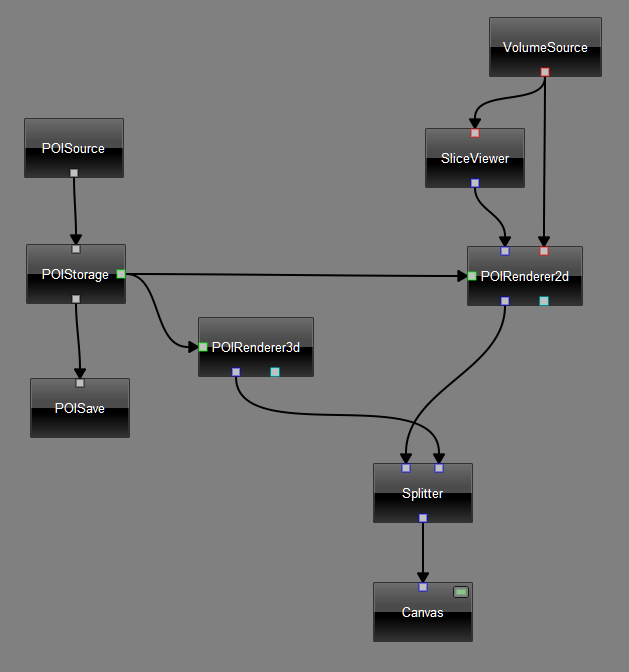
\includegraphics[width=0.8\textwidth]{network.png}
	\caption{Simple POI network}
	\label{fig:network}
\end{figure}

\subsection{Points}
The main objects of the module are the points, which are locations in the 3d (world) space. Each point belongs to a specific group and has an identifications number (id). To insert, and move the points, a \textbf{POIRenderer2d} (see \ref{proc:poirenderer2d}) can be used. 

Groups of points can be selected for modification. Then the \textbf{POISelecionManipulation} processor can   be used to remove them or move them to another group.

\subsection{Groups}
Every point needs to belong to a named group. These groups also define a color for all of their points and can be disabled with all their content at once. They can be managed in the \textbf{POIStorage} (see \ref{proc:poistorage}) processor.

\subsection{VPOI file format}\label{vpoi}
Usually POI data should be stored in the *.vpoi format. It is a custom simple xml format storing the data in the most straightforward way.

\section{Data management processors}
\subsection{POIStorage}\label{proc:poistorage}
The POIStorage is the central processor for every network. It contains and manages all of the POI data. The input port can be used to load data from different sources. If no data is supplied in such a way, an empty list of points and groups is created on initialization. The Output port is used to get the points as a whole object and for example to save them to the disk.

The coprocessor ports are used for all other operations on points. The visualizations need to be connected here. 

The properties, that are used to configure this processor, are shown in the following list:
\begin{itemize}
	\item \textbf{Interaction enabled:} If this is not active, it is not possible to move POI's in the 2d view. It can be used to prevent accidental interactions.
	\item \textbf{Mouseover Point:} If the mouse hovers over a point, this property shows its id, otherwise it is set to -1.
	\item \textbf{Group Configuration:} In the group configuration, groups can be selected, added, and removed with buttons. If a group is selected, its name and color can be changed and it may be enabled or disabled. The currently selected group is also the active group for other processors which use groups (for example it is the group for points placed in the \textbf{POIRenderer2d} (see \ref{proc:poirenderer2d}))
\end{itemize}

\subsection{POISelectionManipulation}
The \textbf{POISelectionManipulation} is used to modify the selected points. They can be moved to a selected group or deleted.

\subsection{POISource}
The \textbf{POISource} is used to load data in the vpoi format (see \ref{vpoi}). It usually should be connected to the \textbf{POIStorage}.

\subsection{POISave}
The \textbf{POISave} processor is used to store the data from files in the vpoi format (see \ref{vpoi}). If the \textbf{Auto save on change} property is checked, it will continuously save the data to the selected file on every change. Otherwise it only stores the data when the \textbf{Save} button is pressed.

\section{Import and Export processors}
\subsection{CSV}
Data can also be stored in CSV (comma seperated values) format. Each row has the format in table~\ref{tab:csv-format}.

\begin{table}[H]
\center

\begin{tabular}{|c|}
\hline 
Integer id \\ 
\hline 
x coordinate in world space \\ 
\hline 
y coordinate in world space \\ 
\hline 
z coordinate in world space \\ 
\hline 
x coordinate in voxel coordinates for some volume \\ 
\hline 
y coordinate in voxel coordinates for some volume \\ 
\hline 
z coordinate in voxel coordinates for some volume \\ 
\hline 
name of the points group \\ 
\hline 
\end{tabular} 
\caption{Line in the CSV file for each point}
\label{tab:csv-format}
\end{table}

\subsection{POICSVImport}
The \textbf{POICSVImport} processor imports data from a CSV file similar to the \textbf{POISource} processor. The coordinates in voxel space are ignored and only the world space positions are used.

\subsection{POICSVExport}
To create CSV files for easy use of the selected data from other software packages, the \textbf{POICSVExport} processor is used. It is similar to the \textbf{POISave} processor, but also needs a volume as its input. The exported voxel coordinates are based on this volume.

\subsection{POIPointListGeometryExporter}
The \textbf{POIPointListGeometryExporter} converts the points to a PointSegmentGeometry, to allow their use with the usual voreen geometry pipeline. For each group, a segment with all of its point is generated.

\subsection{POIPointListGeometryImporter}
The \textbf{POIPointListGeometryImporter} converts a \textbf{PointSegmentListGeometry} to points. The Names of the groups are the segmentnumbers and colors are chosen atomatically.

\section{Rendering processors}
\subsection{POIRenderer2d}\label{proc:poirenderer2d}
The \textbf{POIRenderer2d} is the primary processor for interacting with point data. It depicts points in a slice as colored circles. It is an overlay over a \textbf{SliceViewer}, so its render input port needs to be connected to a slice viewer and the following properties need to be linked to this slice viewer. This is also depicted in figure~\ref{fig:poirenderer2d}.
\begin{itemize}
	\item \textbf{linkedMousePositionInSlice}
	\item \textbf{linkedSliceAlignment}
	\item \textbf{linkedSliceIndex}
	\item \textbf{linkedPickingMatrix}
\end{itemize}
The volume input port needs to get the same volume as the SliceViewer and the processor needs to be connected to a \textbf{POIStorage} with the coprocessor port.

Points can be moved with drag and drop and be placed with Shift \& Click if a group is active in the connected \textbf{POIStorage}.

Points can be selected by dragging a box around them with the mouse. Different modes of selection are avalible.

To configure the processor the following properties are available:
\begin{itemize}
	\item \textbf{Radius in Pixel:} The radius of the circles drawn on the screen
	\item \textbf{Show Arrows:} If this is active, points in other slices are shown as up and down pointing arrows. The direction is the direction in which the mousewheel needs to be turned to scroll to the slice of the corresponding point in usual computer configurations.
	\item \textbf{Max slice distance for arrows:} This sets in how many of the next slices the arrows are drawn. Points in more distant slices are not visible in any way.
	\item \textbf{Show Ids:} This allows to draw a number over every circle with its id number.
	\item \textbf{Font for ids:} The font used to draw the ids over the circles.
	\item \textbf{Color for distance measurement:} If a single point is selected and the mouse hovers over a different point a tool to show this distance is drawn. This is its color.
	\item \textbf{Selection Mode:} Allows to select what happens in case of selection.
	
\end{itemize}

\begin{figure}[H]
	\centering
  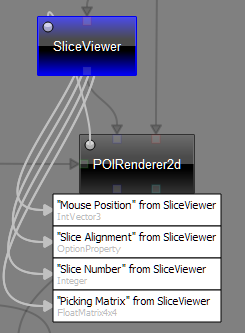
\includegraphics[width=0.4\textwidth]{poirenderer2d}
	\caption{Necessary links between \textbf{POIRenderer2d} and a \textbf{SliceViewer}}
	\label{fig:poirenderer2d}
\end{figure}

\subsection{POIRenderer3d}
The \textbf{POIRenderer3d} renders points as 3d spheres. It is useful to blend it over a 3d rendering of the volume which is being annotated with points. 

Points can be selected by dragging a box around them with the mouse while holding down ALT. Different modes of selection are avalible.

It has the following properties:
\begin{itemize}
	\item \textbf{Autoadjust radius:} If a volume is supplied this enables calculating the radius of the spheres from its diameter
	\item \textbf{Radius:} The radius of each sphere in world space.
	\item \textbf{Radius divider:} If the radius is set to adjust to a supplied volume, the dimension is the volumes diameter divided by this property.
	\item \textbf{Camera:} The camera used for rendering. Usually autolinked by voreen.
	\item \textbf{Color for distance measurement:} See the property with the same name in \textbf{POIRenderer2d} (\ref{proc:poirenderer2d})
\end{itemize}
\subsection{POITextInfo}
The \textbf{POITextInfo} processor writes some general statistics about the groups and and configurable informations its text port.
\begin{itemize}
	\item \textbf{Show group info:} Shows some statistics of the groups before the configurable text.
	\item \textbf{Info text format:} This allows to configure a text. To show some measured quantitys some special tags exists:
	\begin{itemize}
		\item \textbf{\{activeid\}:} Id of the selected points.
	    \item \textbf{\{mouseoverid\}:} Id of the point under the mouse.
	    \item \textbf{\{activegroup\}:} Name of the groups of the selected points.
	    \item \textbf{\{mouseovergroup\}:} Name of the group of the point under the mouse.
	    \item \textbf{\{distance\}:} Distance between the selected point and the point under the mouse.
	    \item \textbf{Selection Mode:} Allows to select what happens in case of selection.
	\end{itemize}
\end{itemize}
\begin{thebibliography}{9}


\bibitem {voreen} Voreen (http://voreen.uni-muenster.de/)
\end{thebibliography}



\end{document}

